% Preview source code

%% LyX 2.1.1 created this file.  For more info, see http://www.lyx.org/.
%% Do not edit unless you really know what you are doing.
\documentclass[english]{article}
\usepackage[T1]{fontenc}
\usepackage[latin9]{inputenc}
\usepackage[a4paper]{geometry}
\geometry{verbose,tmargin=1in,bmargin=1in,headheight=1in,headsep=1in}
\usepackage{float}
\usepackage{amsmath}
\usepackage{graphicx}

\makeatletter

%%%%%%%%%%%%%%%%%%%%%%%%%%%%%% LyX specific LaTeX commands.
%% Because html converters don't know tabularnewline
\providecommand{\tabularnewline}{\\}

\makeatother

\usepackage{babel}
\begin{document}

\title{A Pedestrian Simulation}


\title{Future Virtual Particle Force Model}


\author{Castiglione Gonzalo, Agustin Marseillan, Daniel Parisi}
\maketitle
\begin{abstract}
We present a novel method to simulate virtual pedestrians based on
the social force model. In our model, each pedestrian has a point
in front of him called Future Virtual Particle (FVP) which represents
where the pedestrian is headed to and at what speed.
\end{abstract}
keywords:

pedestrian, collision avoidance, future virtual particle, force model

\pagebreak{}


\section{Introduction}


\subsection{Motivation and previous work}

Navigation of biological, sinthetic or virtual agents is a relevant
problem in several fields such as pedestrian dynamics, moving robots
and animation of characters for videogames and motion pictures.

Modelling and simulating the displacement of agents througth arbitrarily
complex enviroments may be stated in an hierachical structure of mecahnisms
depending mianly on the distance from the agent. This level has been
named, from closer to further, as operational (walking, lowst level
physical-computaitnal model for displacement), tactical (wayfinding,
route chocie) and strategic (general activity planning) {[}Hoogonen
and Bovy 2004{]}. These levels are not independient, factors affecting
one level may impact in the following and vice versa, for example,
the route choice may vary due to congestion of agents producing from
previous route chice and walking behavior. Also, obstacles can impact
on the operational level or tactical level depending on the particular
geometry of the enviroment. The particular mechanism we want to address
is the avoidance of obstacles being fixed or moving (another agent)
which involves operational and tactical aspects of the navigation.

A general approach is to take an existing operational model and equip
it with a higher level model which allows better and smoother collision
avoidance behavior. Exisiting low level models can be taken from pedestrian
dynamics field and in general this models can be classified into rule
based and force based, discrete and continuous space description,
etc. {[}Schadschneider 2009{]}.

A famous example of continuos and force based model is the Social
Force Model {[}Helbing 1995, 2000{]}. In this model the dynamic for
virtual pedestrians is derived from the Newton equation\textquoteright s
considering the total force exceterd over each agent is the result
of three forces: Contact, Social and Driving Force. While the driving
force points towards the final objective of each pedestrian, the social
force is repulsive and acts as a kind of collision avoidance force.
However this social force term introduce several artefacts in some
configurations {[}see for example Lakoba et al. 2005, Parisi et al
2009{]}.

Cellular automata models make use of a spacial grid, which can be
occuied or empty, along with a set of rules determining the evolution
and conflict resolution of virtual pedestrians moving over the cells
of the grid. An emblematic celluar automata model is the one proposed
by Kirchner and Schadschneider {[}2002{]}.

It have been also proposed hibrid models such as the Contractile Particle
Model {[}Baglietto and Parisi, 2011{]} in which a continuos description
of the space is combined with a set of simple rules governig the dynamcis
of the system.

The basic operational model as the ones described above can be improved
if higher level mechanisms were added to manage more complex issues
as eficient avoidance. Some recent examples can be found in the literature.

Karamouzas et al. (2009) proposed a method for collision avoidance
modifying the social force model, basically, replacing the social
force term by a new \textquotedblleft evasive\textquotedblright{}
force which tends to avoid future collisions. The magnitud and direction
of this force is calculaed considering the predictions of these possible
collisions.

Kretz et al. 2011 have arrised the point that the key ingredient in
social force model is the driving force instead of interaction force,
so in this work the authors propose a method for dinamically adjust
the desired velocity following the gradient of a field given by a
time map, in other words, the desired velocity is choosen as the quickest
path to the objective taking into account the geometry and other agents
(collision, congestions, jams, etc.). Also mounted on the SFM, Moussaïd
et al. {[}2011{]} have presented a model using a \textquotedblleft cognitive
heuristics\textquotedblright{} to determine the norm and direction
of the desired velocity for each agent dinamically during the evolution
of the system. 

In the same line, we also proposed that the navigation capacity of
virtual agents should be concentrated in the on-line decision of the
desired velocity. Similar to this approach, we postulate a new method
derived from the methods used in robotics/artificial inteligence\dots{}
The method deals with two aspects of the navigation mechanism. The
first one is geometrical problem of finding intermediate goals when
the final goal is not visible from the current position of the virtual
agent. The second aspect is the local avoidance of other agents, which
is performed via a reactive mechanism inspired in (robot navigation
/ artificial inteligence) aproaches ¿?¿?¿\dots ..?¿?¿ {[} Ref.???
??? {]}. 

The method proposed could be mounted on different basic displacement
models like de SFM or the CPM, in the present work we have chosen
the first one.


\subsection{Social Force Model}

{[}Helbing 1995, 2000{]} presents a Model in which each pedestrian
feels a ``desire force'' towards his objective and a ``repulsion
force'' towards other pedestrians. On a lower level, a collission
force is present.

Collision force (Granular):

\[
F_{G_{i}}=\sum_{j=1,j\ne i}^{N_{P}}[-\epsilon_{ij}k_{n}e_{ij}^{n}+v_{ij}^{t}\epsilon_{ij}k_{t}e_{ij}^{t}]\, g(\epsilon_{ij})
\]


Where: $\epsilon_{ij}=r_{ij}-(R_{i}+R_{j})$

\begin{figure}[H]
\begin{centering}
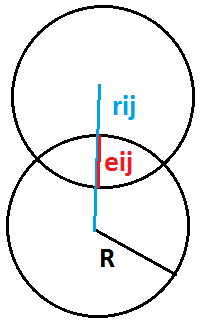
\includegraphics[scale=0.4]{sfm/ganular}
\par\end{centering}

\protect\caption{Fuerza de contact granular}


\end{figure}


\vspace{1cm}


Social Force:
\[
F_{S_{i}}=\sum_{j=1,j\ne i}^{N_{P}}Aexp(-\frac{\epsilon_{ij}}{B})\, e_{ij}^{n}
\]


\vspace{1cm}


\begin{figure}[H]
\begin{centering}
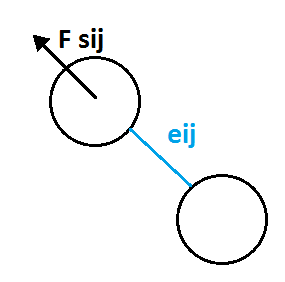
\includegraphics[scale=0.4]{sfm/sf}
\par\end{centering}

\protect\caption{Social Force}
\end{figure}


Desire Force:

\[
F_{D_{i}}=m_{i}\frac{v_{di}e_{i}-v_{i}}{\tau}
\]


\begin{figure}[H]
\begin{centering}
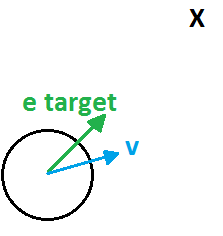
\includegraphics[scale=0.4]{sfm/drivingforce}
\par\end{centering}

\protect\caption{Driving force}
\end{figure}


\vspace{1cm}


Afterwards $F_{i}=F_{G_{i}}+F_{S_{i}}+F_{D_{i}}$is calculated

Fixed parameter values: $A=2000\,[N]$, $B=0.08\,[m]$, $k_{n}=1.2\,10^{5}\,[\frac{N}{m}]$,
$k_{t}=2.4\,10^{5}\,[\frac{kg}{m/s}]$ y $\tau=0.5\,[s]$.

While this model doesn't present a very real behaviour for pedestrians,
it worked as a starting point for numerous projects.


\subsection{Future Virtual Particle Model}

Given that the SFM adds a fictional force on pedestrians, navigation
stops imitating reality when there's a big quantity of pedestrians.
Pedestrians also show a collision avoidance method that resembles
magnetism, with movements that are clearly governed by the squared
distance to the other pedestrian. Also, SFM didn't have the same values
as well known metrics for real-case scenarios such as the flow of
pedestrians going out a door and the fundamental diagram.

Because of this, we present a new model.


\section{The Model}


\subsection{Hipotesis}

The main effects that govern the motion of a pedestrian are the same
as Helbin's:
\begin{enumerate}
\item The pedestrian wants to reach his goal in the shortest possible path.
\item The pedestrian's movement is influenced by other pedestrians. Depending
on the distance between the two of them and the predicted trayectory,
the pedestrian will feel the need to change his route to be able to
avoid the other pedestrians. It is because of this effect that pedestrians
will need to recalculate their route as new pedestrians get closer
to them.
\item Movement speed will be influenced by needs.
\end{enumerate}

\subsection{Definition}

A pedestrian is defined as follows:
\begin{itemize}
\item Circular shape


Represents the space that this pedestrian occupies. Circle's radio
is generated randomly to represent different types of pedestrians.
The range of values is distributed uniformly in $[0.25,0.29]$$[cm]$.

\item Long term objective


Represented by a static area. When it is touched by a pedestrian,
it is considered as accomplished. Multiple objectives can by defined
in a list, in this case, each of them must be reached in order.

\item Short term objective


Called FVP, it represents a point at a relative distance from the
pedestrian's center. It's a dynamic objective.


It is defined as a$1$ $[kg]$ mass. Not collisionable.

\item Desired speed


Represents the speed the pedestrian would walk if he was alone. Varies
randomly between$[1.2,1.4]$ $[m/s]$.

\item Reaction distance 


Maximum distance between a pedestrian and his FVP, it represents the
distance at which a real pedestrian would react from an obstacle.

\end{itemize}
\vspace{1cm}


Fig 1: Pedestrian and his FVP.

\begin{figure}[H]
\centering{}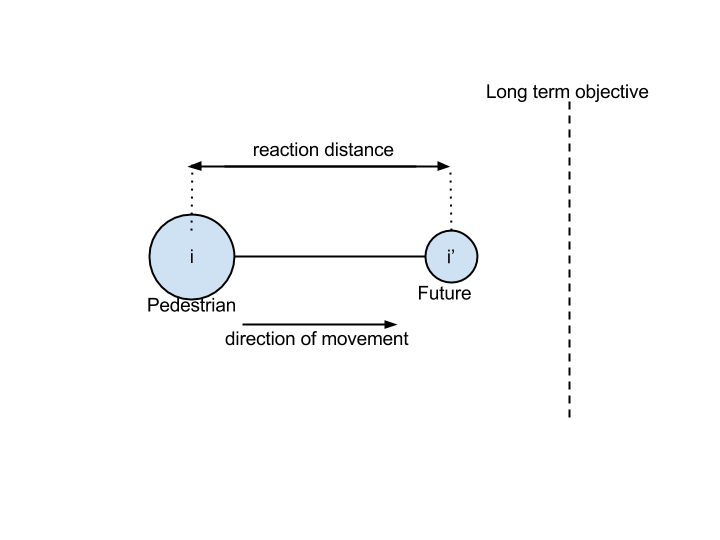
\includegraphics[scale=0.5]{pedestrian-top}\protect\caption{Pedestrian top view}
\end{figure}


In the document, we will call pedestrians with a letter and FVP of
pedestrian x will be called x'.\\



\subsection{Algorithm}

Each pedestrian has to reach the long term objective at some point,
to ensure this, the FVP always feels the need to be aligned with the
shortest path to the long term objective. On the other hand, there
are sometimes obstacles in the way, which will make this impossible,
in this cases, the route will have to change depending on the situation.

The pedestrian movement is calculated in four steps:
\begin{enumerate}
\item Calculate forces for each FVP.
\item Update positions for each FVP.
\item Calculate forces for each pedestrian.
\item Update positions for each pedestrian.\\

\end{enumerate}
Each step is defined as follows:
\begin{enumerate}
\item FVP force calculation. 


In each iteration, the FVP from pedestrian $i$ feels a force generated
by the other pedestrians and FVPs. First of all, we filter de pedestrians
$j$ who are not in the range of sight of pedestrian $i$ as follows:


\[
k=i+\begin{pmatrix}0 & -1\\
1 & 0
\end{pmatrix}\overrightarrow{ii'}
\]
The following must be valid:


\[
(k_{x}-i_{x})*(j_{y}-i_{y})-(k_{y}-i_{y})*(j_{x}-i_{x})>0
\]



Once filtered, the force is calculated for every other FVP. The repulsion
force between i' and j' is defined as follows:


\[
F_{ext}(i)=\sum_{j}F_{i',j'}=\sum_{j}\alpha e^{-dist(i',j')/\beta}
\]



where $\alpha$ and $\beta$ are predefined constants. Afterwards,
we calculate the repulsion force between i' and j using the same formula
but different $\alpha$ and $\beta$. Afterwards, we calculate the
force between pedestrian i and his FVP i', this is a force that pushes
i' to be in its desired relative distance from the pedestrian. This
force is represented with a spring of length ``reaction distance''
and constant $K$. When we sum all these, we get the final $F_{ext}$.


Fig 2: FVP force calculation.


\begin{figure}[H]
\centering{}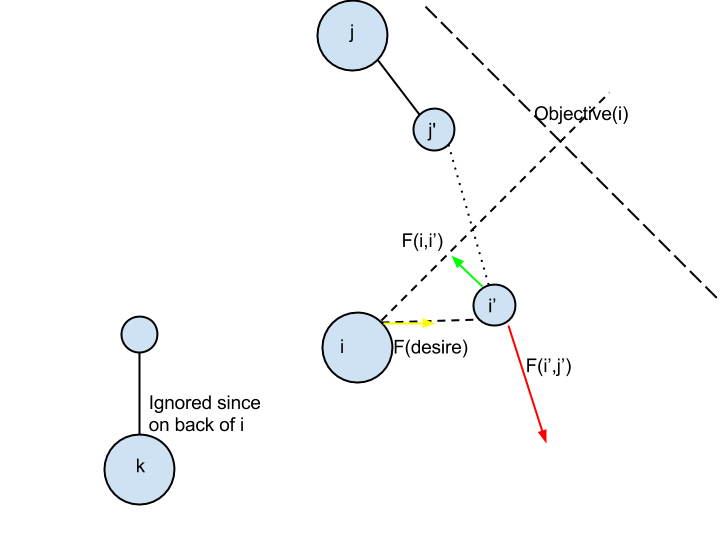
\includegraphics[scale=0.5]{pedestrian-top-forces}\protect\caption{Fuerzas que actúan sobre el Future $i'$}
\end{figure}

\begin{enumerate}
\item FVP position update.


In this stage, the position of the FVP is updated with Euler's formula
and the forces calculated in the previous step.

\end{enumerate}

To avoid high simetry situations, a low noise $P=10\%$ is added to
$F$. There are two ways to apply this noise:
\begin{itemize}
\item Radial noise:

\begin{itemize}
\item A value $p$ is taken randomly from a uniform distribution $[-P,\, P]$
and calculate: $FL_{i'}=F_{i'}*p$
\item Angular noise:

\begin{itemize}
\item A value $sgn=\{-1,\,1\}$ is taken randomly from a uniform distribution
and a value $p$ from $[-P,\, P]$. Then $FA_{i'}=rotation(F_{i'},\,\pi*sgn)*p$
is calculated.
\end{itemize}
\end{itemize}

At last, we find $F'_{i'}=F_{i'}+FL_{i'}+FA_{i'}$ and apply euler's
movement equations.

\end{itemize}
\begin{enumerate}
\item Pedestrian forces calculation. 


The pedestrian always wants to move in the direction his FVP is pointing
and its magnitude is defined as Fd or desire force:

\end{enumerate}

\[
F_{desire_{i}}=m_{i}\frac{\frac{dist(i',i)}{dist_{react}}e_{i}-v_{i}}{\tau}
\]



Where $\tau=0.5$
\begin{enumerate}
\item Pedestrian position update. 


The new position of the pedestrian will be calculated using Euler's
formula and the desire force calculated in the previous step.

\end{enumerate}
\end{enumerate}

\section{Calibration}


\subsection{Metrics}

The results where compared to the SFM using the values propposed by
Dirk Helbing {[}2{]}. The test scenarios where crossing and hallway
for they present the main two types of simmetry (90 degrees and 180
degrees).

The metrics used where:
\begin{enumerate}
\item Number of collisions


When a pedestrian's body is touching another one, a counter is incremented,
it won't be incremented again unless it separates and touch again.
This counter represents the amount of collisions.

\item Total duration of collisions:


When a pedestrian's body is touching another one, a counter is incremented
by the time step of the simulation. This counter will represent the
total time pedestrians were colliding.

\item Average walking speed:


//TODO

\item Average travel time:


When a pedestrian appears in the map, this time is recorded, once
he reaches his goal, the travel time is calculated with this value.
The average of all this times represents the average travel time.

\item Average travel distance:


Each step, the distance a pedestrian has traveled from the source
is saved. When this pedestrian reaches his goal, that distance is
considered as finished and it is saved elsewhere. Afterwards, an average
of all finished distances is calculated.

\item Average turn angle:


Each step, the angle of the previous velocity of a pedestrian and
the current one is saved and added to a total. When this pedestrians
reaches his goal, this total is considered as finished and it is saved
elsewhere. Afterwards, an average of all finished turn angles is calculated.

\end{enumerate}

\subsection{Values}

To calibrate the model, runs varying parameters were made. A wide
spectrum of values was covered, testing every combination of every
possible one. After seeing clear preferences towards certain values,
the values were refined within that scope. After numerous iterations
of this process, the values that best suit these metrics are$\alpha=800$
y $\beta=[0.65,\,085]$ uniformly distributed.

//TODO todos los demás parámetros


\section{Results}

\vspace{1cm}


\begin{table}[H]
{\scriptsize{}}%
\begin{tabular}{|c|c|c|c|c|c|c|}
\hline 
{\scriptsize{}Values} & {\scriptsize{}1} & {\scriptsize{}2} & {\scriptsize{}3} & {\scriptsize{}4} & {\scriptsize{}5} & {\scriptsize{}6}\tabularnewline
\hline 
\hline 
{\scriptsize{}$\alpha=800,\,\beta=[0.65,\,0.85]$} & {\scriptsize{}(1.800, 0.748) } & {\scriptsize{}(34.600, 8.333) } & {\scriptsize{}(1.024, 0.016) } & {\scriptsize{}(1.910, 0.022) } & {\scriptsize{}(2.392, 0.005) } & {\scriptsize{}(111.062, 19.122)}\tabularnewline
\hline 
{\scriptsize{}$\alpha=2000,\,\beta=0.08$} & {\scriptsize{}(5.333, 2.625)} & {\scriptsize{}(12.333, 8.340) } & {\scriptsize{}(1.052, 0.003) } & {\scriptsize{}(1.876, 0.003) } & {\scriptsize{}(2.391, 0.002) } & {\scriptsize{}(106.185, 13.778)}\tabularnewline
\hline 
\end{tabular}\protect\caption{Metrics comparing SFM vs FVPM. Average of $10$ runs.}
\end{table}




\textbf{// Poner Graficos indicando distancias y esquemas del future
y la particula. }


\section{Conclusions}

\textbf{// agregar al final futuras opciones que se abren con este
trabajo}

\pagebreak{}


\section{References}
\begin{itemize}
\item {[}1{]} ... Karamouzas ...
\item {[}2{]} ...Helbing ...\end{itemize}

\end{document}
